\chapter{Background}
\label{background}
\section{Existing alternatives}
As of writing this thesis, only very few tools support monitoring of STP topologies.
The ones we found are LoriotPro\cite{LoriotPro}, LiveAction\cite{LiveAction} and L2Discover\cite{L2Discover}.
Of these three network monitoring tools, only L2Discover has its source code openly available.
The company SolarWinds has an open vote on their website on whether or not to include this feature in their monitoring software since 2014\cite{thwackSW}.
LoriotPro and L2Discover use the SNMP for their topology discovery, with STP only being used to discover duplicate and unused links.
\tool\ uses only STP, thus not needing the networking hardware being SNMP capable.

While commercial tools mostly use active methods for network discovery, several research projects have also attempted to develop purely passive or hybrid tools.
One of the first of these tools was developed by Becker et al.\cite{becker1995} in 1995.
In more recent years, Blue et al.\cite{blue2008} and Wongsuphasawat et al.\cite{wongsuphasawat2009} published papers on passive network visualization tools in 2008 and 2009.
However, not much work has been done on purely passive STP visualization.

\section{Spanning Tree Protocol (STP)}
\label{stp}
\subsection*{Port States}
The most important part of STP is its introduction of port states.
These port states ensure that the spanning tree does not contain loops.
Ports can be in one of three states (see Figure~\ref{fig:port_states}):
\begin{itemize}
    \item \textcolor{green}{\textbf{Root Port}}: the port leading to the root or "upwards" in the tree.
        Every non-root bridge has \textbf{exactly one} root port.
    \item \textcolor{blue!80}{\textbf{Dedicated Port}}: dedicated ports are ports where packets are sent. These are the ports leading "downward" in the tree.
        The root has only dedicated ports.
    \item \textcolor{red}{\textbf{Blocking Port}}: no packets are sent via a blocking Port.
        This state is used to disable alternate paths to the root or "sideways" in the tree.
\end{itemize}
In the original STP paper\cite{perlman85}, the term Local Area Network (LAN) referred to any connection to a bridge, as well as between bridges.
Because the STP information must be propagated to every LAN, there needs to be exactly one dedicated port in a LAN.
In a LAN between two non-root bridges, the bridge with the smaller root path cost (see Figure~\ref{fig:stp_bpdu}) will make its connected port dedicated.
Should both bridges have the same path cost to the root, the one with the smaller bridge identifier becomes the dedicated bridge (see Section~\ref{stp_packet}: STP Packets).
This can be seen in the connection between the bottom bridges in Figure~\ref{fig:port_states}.
If no superior STP packets are received on a blocking or root port for a set amount of time (called the forward delay) it transitions to the dedicated state.
\begin{figure}[h]
    \centering
    \begin{tikzpicture}
        \node (root) at (2,2) {\switch{0.8}{Root}};
        \node (a) at (0,0) {\switch{0.8}{A}};
        \node (b) at (4,0) {\switch{0.8}{B}};

        \draw
        (root) -- node[dedicated, at start]{} node[root, at end]{} (a)
        (root) -- node[dedicated, at start]{} node[root, at end]{} (b)
        (a) -- node[dedicated, at start]{} node[blocking, at end]{} (b);

        \begin{customlegend}[legend cell align=left, legend entries={Root Port,Dedicated Port,Blocking Port},
            legend image post style={scale=2.3},
            legend style={at={(8,2)},font=\footnotesize}]
            \addlegendimage{white,mark=*,fill=green}
            \addlegendimage{white,mark=*,fill=blue!80}
            \addlegendimage{white,mark=*,fill=red}
        \end{customlegend}
    \end{tikzpicture}
    \caption{An example of STP port states}
    \label{fig:port_states}
\end{figure}

\subsection*{STP Packets}
\label{stp_packet}
In this section we will explain the individual fields in an STP Bridge Protocol Data Unit (BPDU), as seen in Figure~\ref{fig:stp_bpdu}.
\begin{figure}[h]
    \centering
    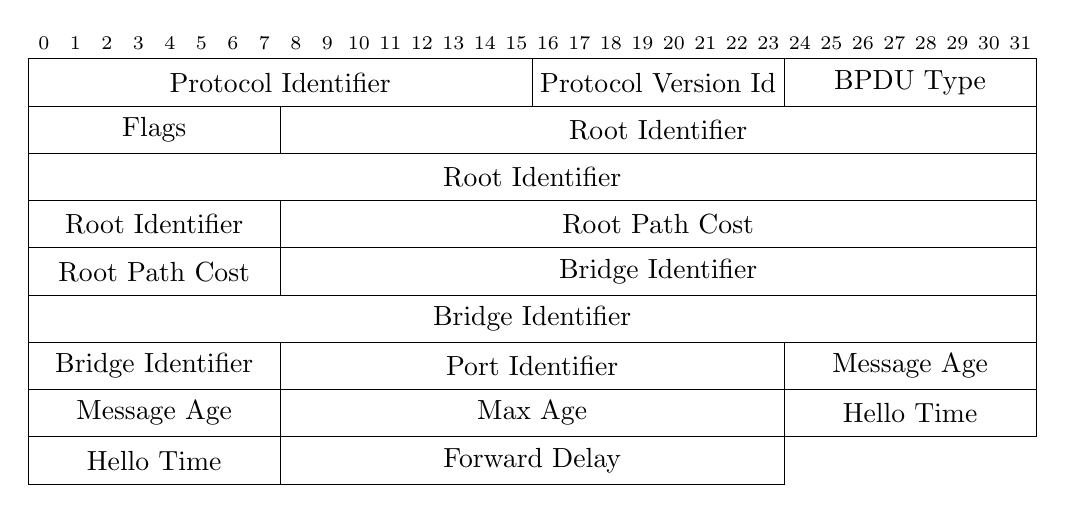
\begin{tikzpicture}[scale=0.4]
        \foreach \x in {0,...,31}
            \node at (\x+0.5,20.5) {\scriptsize \x};
        \draw (0,20) rectangle (16,18.5); \node (mode) at (8, 19.25) {Protocol Identifier};
        \draw (16,20) rectangle (24,18.5); \node (mode) at (20, 19.25) {Protocol Version Id};
        \draw (24,20) rectangle (32,18.5); \node (mode) at (28, 19.25) {BPDU Type};
        \draw (0,18.5) rectangle (8,17); \node (mode) at (4, 17.75) {Flags};
        \draw (8,18.5) rectangle (32,17); \node (mode) at (20, 17.75) {Root Identifier};
        \draw (0,17) rectangle (32,15.5); \node (mode) at (16, 16.25) {Root Identifier};
        \draw (0,15.5) rectangle (8,14); \node (mode) at (4, 14.75) {Root Identifier};
        \draw (8,15.5) rectangle (32,14); \node (mode) at (20, 14.75) {Root Path Cost};
        \draw (0,14) rectangle (8,12.5); \node (mode) at (4, 13.25) {Root Path Cost};
        \draw (8,14) rectangle (32,12.5); \node (mode) at (20, 13.25) {Bridge Identifier};
        \draw (0,12.5) rectangle (32,11); \node (mode) at (16, 11.75) {Bridge Identifier};
        \draw (0,11) rectangle (8,9.5); \node (mode) at (4, 10.25) {Bridge Identifier};
        \draw (8,11) rectangle (24,9.5); \node (mode) at (16, 10.25) {Port Identifier};
        \draw (24,11) rectangle (32,9.5); \node (mode) at (28, 10.25) {Message Age};
        \draw (0,9.5) rectangle (8,8); \node (mode) at (4, 8.75) {Message Age};
        \draw (8,9.5) rectangle (24,8); \node (mode) at (16, 8.75) {Max Age};
        \draw (24,11) rectangle (32,8); \node (mode) at (28, 8.75) {Hello Time};
        \draw (0,8) rectangle (8,6.5); \node (mode) at (4, 7.25) {Hello Time};
        \draw (8,8) rectangle (24,6.5); \node (mode) at (16, 7.25) {Forward Delay};
    \end{tikzpicture}
    \caption{An STP BPDU}
    \label{fig:stp_bpdu}
\end{figure}\\
The fields we used for \tool\ are:
\begin{itemize}
    \item \textbf{Flags}: The flags byte is used for the \textit{topology change (TC)} and \textit{topology change acknowledgement (TCA)} flags.
    \item \textbf{Root/Bridge Identifier}: The Identifier consists of three parts and has the same layout for the root and regular bridges:
        \begin{itemize}
            \item Priority (4 Bits): A value between 0 and 61440 configurable in increments of 4096
            \item System ID Extension (12 Bits): Used for keeping the bridge ID unique if multiple VLANs are configured for a bridge
            \item Bridge MAC (6 Byte): The MAC address of the bridge
        \end{itemize}
        The conjunction of these three parts is used in comparisons as one large 8 byte number.
    \item \textbf{Root Path Cost}: The root path cost is the sum of all port costs (which can be configured in the bridge) along the current path. The root path cost in packets sent by the root is 0.
    \item \textbf{Message Age}: The message age is the number of bridges that have been passed (in addition to the root) along the current path.
    \item \textbf{Max Age}: If the message age surpasses this maximum, packages are not forwarded any more.
    \item \textbf{Hello Time}: The delay in seconds between sent \textit{Hello} BPDUs.
        \textit{Hello} BPDUs have the form shown in Figure~\ref{fig:stp_bpdu}.
    \item \textbf{Forward Delay}: After this time, if no superior packet was received, a root, or blocking port will transition to dedicated.
        Note that if a root port transitions to dedicated state that means the bridge now assumes it is the root.
\end{itemize}
A BPDU only contains information about the root and the bridge that sent the package.
This means that if there is a bridge between these two, we will not know about its ID.
We will however still know that it is there, because of the message age.
During the buildup of the tree it is possible to obtain information on intermediate nodes.
This possibility is explained more in-depth in the section on packet handling (Section~\ref{packet_handling}).

\subsubsection*{Default Parameters}
The parameters discussed default to the following values\cite{params}:
\begin{itemize}
    \item \textbf{Priority}: 32768
    \item \textbf{System Id Extension}: 0
    \item \textbf{Max Age}: 20
    \item \textbf{Forward Delay}: 15
    \item \textbf{Hello Time}: 2
\end{itemize}

\subsection*{Spanning Tree Algorithm}
The original paper on STP does not describe an algorithm itself, it merely lists constraints that have to be fulfilled.
Algorithm~\ref{alg:stp} shows the algorithm we use in our own \textit{software-switch} testing tool.
We use a reduced number of port states, ignoring the transition states, by utilizing the timestamps of received BPDUs.
The algorithm's purpose is to keep loops out of the network, as well as keeping the tree topology consistent.

\begin{algorithm}[h]
    \DontPrintSemicolon
    \KwData{\\
    $received$ = received packet\;
    $current$ = data of the current bridge\;
    }
    \;
    \If{$received.rootId < current.rootId$}{
        \tcc{There is a new root in the network}
        $current.rootId=other.rootId$\;
        set receiving port as root-port\;
        set other ports to dedicated\;
    }{
        \uIf{$received.rootPathCost<current.rootPathCost$}{
            \tcc{This means that the path via the other bridge is shorter, so this should be our new root-path}
            set receiving port as root-port\;
            set other ports to dedicated\;
        }
        \ElseIf{$received.rootPathCost==current.rootPathCost \land received.bridgeId<current.bridgeId$}{
            \tcc{Both bridges are equidistant from the root, but the other bridge has a lower bridge Identifier and should be the dedicated bridge on the connection}
            set receiving port as blocking port\;
        }
        \tcc{Check if the transitions described in the section on \textbf{STP Packets} are necessary}
        doPacketTimeOutTransitions()\;
    }
    
    \caption{Spanning Tree Algorithm (STA)}
    \label{alg:stp}
\end{algorithm}

\subsection*{Extensions}
Since the inclusion of STP in the IEEE 802.1D\cite{802.1D} standard, multiple additions have been made to the STP.
Rapid STP (RSTP) has been developed to decrease the time needed for tree convergence.
Per VLAN STP (PVSTP) has been developed by Cisco and is a proprietary variant which allows for multiple spanning trees to exist, one for each VLAN.
The Multiple STP (MSTP) is an extension of RSTP which, like PVSTP, allows for multiple spanning trees to exist in their own VLAN.
In addition to that, it also allows for VLAN specific trees to be combined into one large spanning tree.

As an extension to STP the Shortest Path Bridging (SPB)\cite{spb} protocol was developed.
It allows for multiple paths to be active at the same time, and uses global information to allow for the calculation of shortest paths.

While the aforementioned extensions to STP would make our task a lot easier (especially SPB), they are not as prevalent as basic STP (which most switches are capable of).
For this reason we decided to confine our efforts to basic STP.

\section{Technologies used}
\subsection*{PCAP}
\label{pcap}
PCAP\cite{pcap} is a shortening of packet capture.
It used to be a part of the \textit{tcpdump} tool before it was pulled into it's own library.
We used the UNIX version \textit{libpcap} for this thesis.
\textit{Libpcap} is a C library and can be directly linked with C and C++ without using a wrapper.
It provides functions for opening live network devices and \textit{.pcapng} files.
After starting a live capture on a device, \textit{libpcap} will call a callback function for every packet received on the opened interface.
The prototype of the callback function looks as follows:
\begin{lstlisting}[caption=Pcap Callback Prototype]
typedef void (*pcap_handler)(u_char *user, const struct pcap_pkthdr *h, const u_char *bytes);
\end{lstlisting}
Where the parameters are:
\begin{itemize}
    \item \textbf{u\_char *user} is used to pass user defined parameters.
    \item \textbf{pcap\_pkthdr *h} contains useful information about the packet, like source and destination addresses, as well as size.
    \item \textbf{u\_char *bytes} contains the actual (binary) data of the packet.
\end{itemize}
The \textbf{typedef void} (*pcap\_handler) part of the prototype just means that the function returns a \textbf{void *}.

Usage of this function will be covered more in-depth in the chapter on \tool itself (Chapter~\ref{stp-gen}).
\subsection*{JSON}
\label{json}
JSON stands for Java Script Object Notation and was used for two reasons:
\begin{enumerate}
    \item It keeps the network communication independent from any programming languages used.
    \item Utility libraries for JSON are easily available for most programming and scripting languages, saving us the work of inventing and implementing our own notation.
\end{enumerate}
JSON has a simple notation for declaring objects and arrays, as well as primitive data types.
An example is shown in Listing~\ref{lst:json}.
\lstinputlisting[caption=JSON Example, label=lst:json]{../listings/json/example.json}
The JSON library used in this thesis is \textit{jsoncpp}\cite{jsoncpp}.

\subsection*{TikZ}
\label{tikz}
We chose TikZ ist kein Zeichenprogramm (TikZ)\cite{tikz} as the file format for our output.
Using TikZ allows us to generate \textit{.tex} files rather than images.
These are easier to generate, as well as to modify after creation.
It is also very easy to integrate in \LaTeX\ papers.
While TikZ is very powerful and therefore complex, the parts we use are fairly simple.
Listing~\ref{lst:tikz_example} shows the TikZ code for Figure~\ref{fig:bc_storm_b}.
\lstinputlisting[caption=A TikZ Example, label=lst:tikz_example]{../listings/tikzExample.tex} %TODO: check positioning
The \textbackslash node keyword draws a node with the id given in parenthesis.
It is centered around the coordinates given with the \textit{at} keyword and has the text written in braces.
The (0,0) coordinate is in the top left corner of an image.
For our graphics we used a self defined \textbackslash switch macro, but regular text or \LaTeX\ commands work as well.
Edges are drawn using the \textbackslash draw command.
This command can be used with raw coordinates or identifiers.
Options for the edges can be passed in brackets.
Note that \textit{edge} can be substituded with \textit{- -}.
All TikZ commands are ended with a semicolon.
TikZ graphics are automatically cropped on rendering.

